\documentclass[10pt,twocolumn]{article}

\usepackage{times}
\usepackage{mathptmx}  
\usepackage{spverbatim}
\usepackage{fixltx2e}
\usepackage[utf8]{inputenc}
\usepackage{graphicx}
\usepackage{sidecap}
\usepackage{fancyhdr}
\usepackage{amssymb,amsmath}
\usepackage[swedish]{babel}
\usepackage[margin=1.5in]{geometry}
\usepackage{abstract}
\usepackage[parfill]{parskip}
\usepackage{tocloft}
\usepackage{adjustbox}
\usepackage{textcomp}
\usepackage[T1]{fontenc}
\usepackage{listings}
\usepackage{xcolor,colortbl}
\usepackage{hyperref}
\usepackage{mcode}
\usepackage{a4wide}
\usepackage{caption}
\usepackage{epstopdf}

\raggedbottom
\sloppy

\title{Laborationsrapport i TSKS10 \emph{Signaler, Information och Kommunikation}}

\author{Hans-Filip Elo, hanel742, 900109-5174}

\begin{document}

\maketitle

\section{Inledning}

Vid kommunikation används ofta I-/Q-modulering för att överföra en signal inom ett givet frekvensutrymme. I och med överföringen kan tidsfördröjningar införas. I mottagaränden måste dessa tidsfördröjningar kompenseras för innan överföringen sedan kan I-/Q-demoduleras för att extrahera ljudinformationen 

\subsection{Syfte}

Syftet med denna laboration är att finna bärfrekvens för en given signal, filtrera bort oönskade delar av överföringen och sedan I-/Q-demodulera signalen för att extrahera relevant information. 

\subsection{Materiel och förutsättningar}

Filen signal-hanel742.wav är given med den kända samplingsfrekvensen 400 kHz. Givet är också att filen innehåller en smalbandig signal som är I-/Q-modulerad och har skickats genom filtret nedan. 

\begin{gather}
h(t) = \delta(t - \tau_1) + \delta(t - \tau_2)
\label{equ:filter}
\end{gather}

På förhand ges också att bärfrekvensen för relevant del av signalen är en multipel av 19 kHz.

Signalen innehåller två melodier samt två olika ordspråk. 

För att utföra laborationen används GNU Octave med vertygslådor för ljud samt signaler (octave-audio och octave-signal) installerat. 

% -------- Metod ------------
\section{Metod}

Jag börjar med att läsa in filen i Octave och sedan fouriertransformera signalen för att få ut dess frekvensspektrum: 

\begin{figure}[htp]
  \begin{center}
  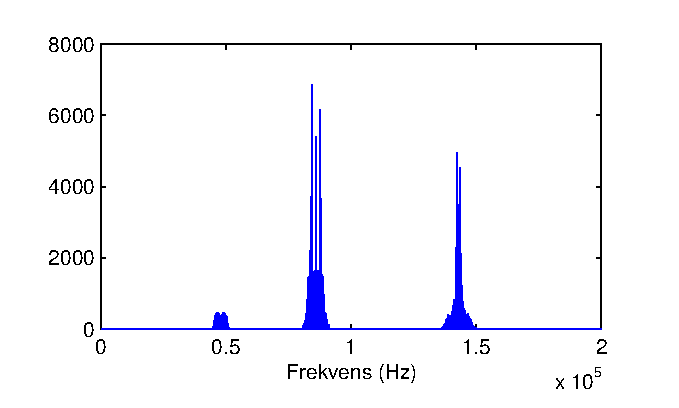
\includegraphics[keepaspectratio=true,width=\linewidth]{fft_orig_data_oneside.eps}  %skala och filnamn. 
  \end{center}
  \caption{Enkelsidigt amplitudspektrum för ursprunglig signal} %figurtext.
  \label{fig:fft_orig_data}
\end{figure}

\subsection{Att finna bärfrekvensen}

Jag vill nu filtrera ut signalelementen för de olika topparna ur totala signalen. För att göra detta använder jag tre olika bandpassfilter med gränsfrekvenserna $[40000, 80000]$, $[100000, 130000]$ samt $[140000, 160000]$.

Genom att utläsa frekvenserna ur topparna i figur~\ref{fig:fft_orig_data} kan man se att topparna har bärfrekvenser i området kring frekvenserna i tabell \ref{table:carryfreq}. Topparna räknas från origo och utåt och filtrens gränsfrekvens anges till höger i tabellen. 
\begin{center}
\begin{tabular}{c | c }
	\hline
	Topp & Ungefärlig bärfrekvens (Hz) \\ \hline
	1 & $4,959 \cdot 10^4$ \\ \hline
	2 & $8,313 \cdot 10^4$ \\ \hline
	3 & $1,412 \cdot 10^5$ \\ \hline
\end{tabular}
\captionof{table}{B{\"a}rfrekvenser} \label{table:carryfreq}
\end{center}
Filtrerar man sedan den givna signalen med hjälp av bandpassfilter med givna gränser ges utseende enligt figurer i appendix A. Enligt utseendet på graferna ser frekvenstopp i figur~\ref{fig:topp1_filter} ut att innehålla någon form av information, medan toppen i figur~\ref{fig:topp3_filter} mest verkar innehålla vitt brus. 

Frekvenstoppen i figur~\ref{fig:topp2_filter} är mer svårbedömd - men en rimlig uppskattning är att den har ett alldeles för periodiskt utseende för att innehålla någon intressant information. 

Närmsta multipel av 19 kHz för den uppskattade bärfrekvensen, $f_c$, för frekvenstoppen i figur~\ref{fig:topp1_filter} är 57 kHz, vilket väljs till bärfrekvens för fortsatta experiment. 

\subsection{Filtrering}

När signalen skickas genom filtret givet i uppgiften skapas ett eko med styrkan $90\%$ av ursprungliga signalen. Detta eko har en tidsfördröjning som är lika med beloppet av differensen av filtrets två tidsfördröjningar, alltså $|\tau_1 - \tau_2|$.

Fördröjningen ges relativt enkelt ur mångtydighetsfunktionen för det vita bruset som syns i figur~\ref{fig:topp3_filter}. Detta ger tre tydliga toppar ur vilka man kan utläsa tidsfördröjningen. 
\begin{figure}[htp]
  \begin{center}
  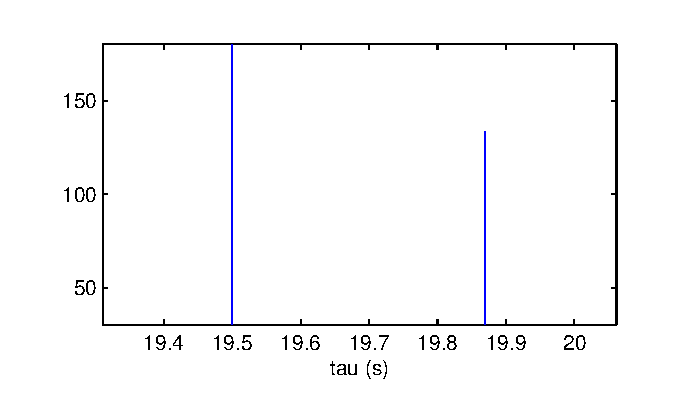
\includegraphics[keepaspectratio=true,width=\linewidth]{xCorr.eps}  %skala och filnamn. 
  \end{center}
  \caption{Mångtydighetsfunktion för vitt brus} %figurtext.
  \label{fig:xCorr}
\end{figure}
Mätningar ur figur \ref{fig:xCorr} ger att tidsfördröjningen är lika med $370\;ms$. 

Då vi samplar med en frekvens av $400 000\;Hz$ ges tidsfördröjningen $|\tau_1 - \tau_2|$ i antal samples (n) enligt nedan 

\begin{gather}
n = 0,370 \cdot 400 000 = 148 000
\label{equ:delaySamples}
\end{gather}
Innan man kan I-/Q-demodulera signalen behöver det eko som uppstår då signalen passerar det givna filtret tas bort. 

De första $n$ antal samples innehåller inget eko. Nästkommande $n$ samples innehåller eko som kan tvättas bort med förstkommande $n$ samples. När $n+n$ samplingar är fria från eko kan man använda samplingar $n-(2n-1)$ för att tvätta bort eko från nästkommande $n$ samples. Processen upprepas tills dess att hela signalen är fri från eko. Ett steg i processen utförs alltså enligt nedan

\begin{gather}
S_{utan eko}^{aktuell} = S_{eko}^{aktuell} - 0,9S_{utan eko}^{tidigare}
\label{equ:eko}
\end{gather}

\subsection{I-/Q-demodulation}

För att demodulera signalen används principer som beskrivs av Erik G. Larsson (2014). I- och Q-komponenter ges enligt nedan: 

\begin{gather}
x_{I}(t) = \Large{H}_{B/2\;Hz}^{LP}\{2x(t)\cos{(2{\pi}f_{c}t + \theta)}\} \\
x_{Q}(t) = -\Large{H}_{B/2\;Hz}^{LP}\{2x(t)\sin{(2{\pi}f_{c}t + \theta)}\}
\label{equ:iq}
\end{gather}

Där $\theta$ är fasförskjutningen. Fasförskjutningen har tyvärr testats fram då möjligt område för den är relativt litet, $[0,\frac{\pi}{2}]$, och det vad undertecknad vet ej finns något sätt att entydigt bestämma fasförskjutningen. Fasförskjutningen kan endast vara i området $[0,\frac{\pi}{2}]$ då I- och Q- demoduleringen sedan växlar plats på informationen - i o m egenskaper hos $\cos$ och $-\sin$. Fasförskjutningen då meddelandet framgår bäst bestämdes till $0$.


% -------- Slutsatser ------------
\section{Resultat och slutsats}

Funna egenskaper hos signalen är: 

\begin{itemize}
	\item $f_c = 57$ kHz
	\item $|\tau_1 - \tau_2| = 370$ ms
\end{itemize}

Först spelas två melodier - varav en blinka lilla stjärna. Sedan hörs två ordsspråk. Ordspråken som hörs är: 

\begin{itemize}
	\item ''Man kan inte både ha kakan och äta den''
	\item ''Man ska inte säga Hin i död mans hus''
\end{itemize}
% -------- Appendix ---------------

\appendix
\pagestyle{empty}
\newgeometry{left=2cm,right=2cm,bottom=2cm,top=2cm}
\section{Filtrerade signaler}

\begin{figure}[htp]
  \begin{center}
  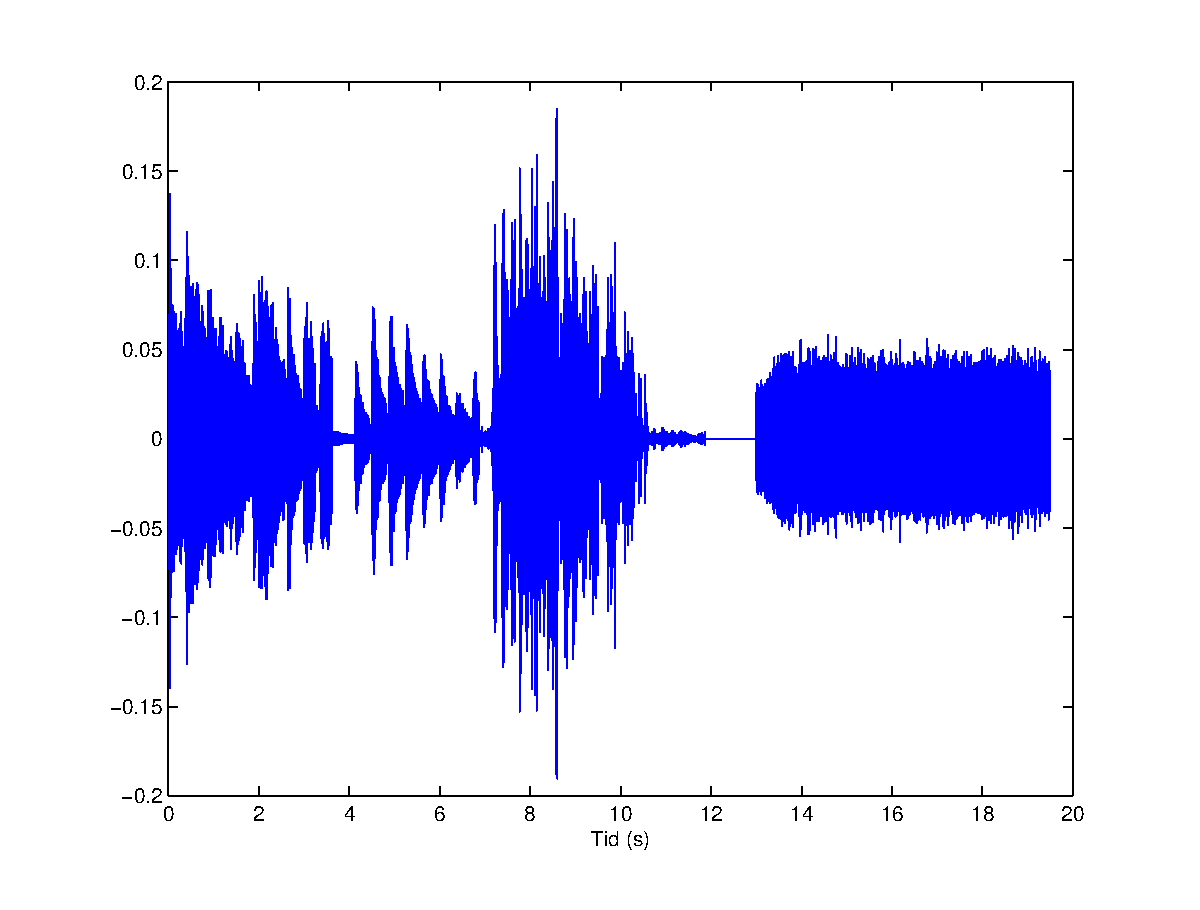
\includegraphics[keepaspectratio=true,width=\linewidth]{topp1_filter.eps}  %skala och filnamn. 
  \end{center}
  \caption{Frekvenstopp 1 filtrerad} %figurtext.
  \label{fig:topp1_filter}
\end{figure}

\begin{figure}[htp]
  \begin{center}
  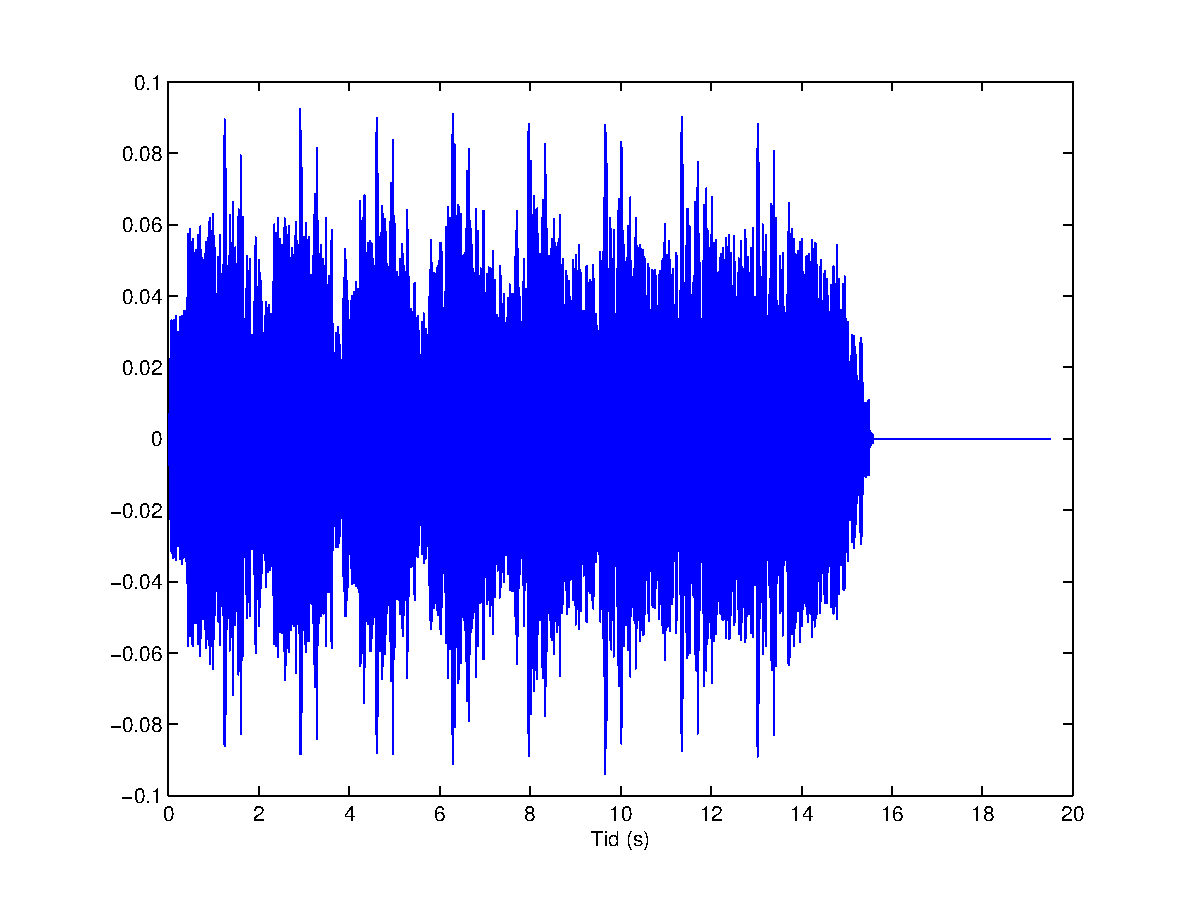
\includegraphics[keepaspectratio=true,width=\linewidth]{topp2_filter.eps}  %skala och filnamn. 
  \end{center}
  \caption{Frekvenstopp 2 filtrerad} %figurtext.
  \label{fig:topp2_filter}
\end{figure}

\begin{figure}[htp]
  \begin{center}
  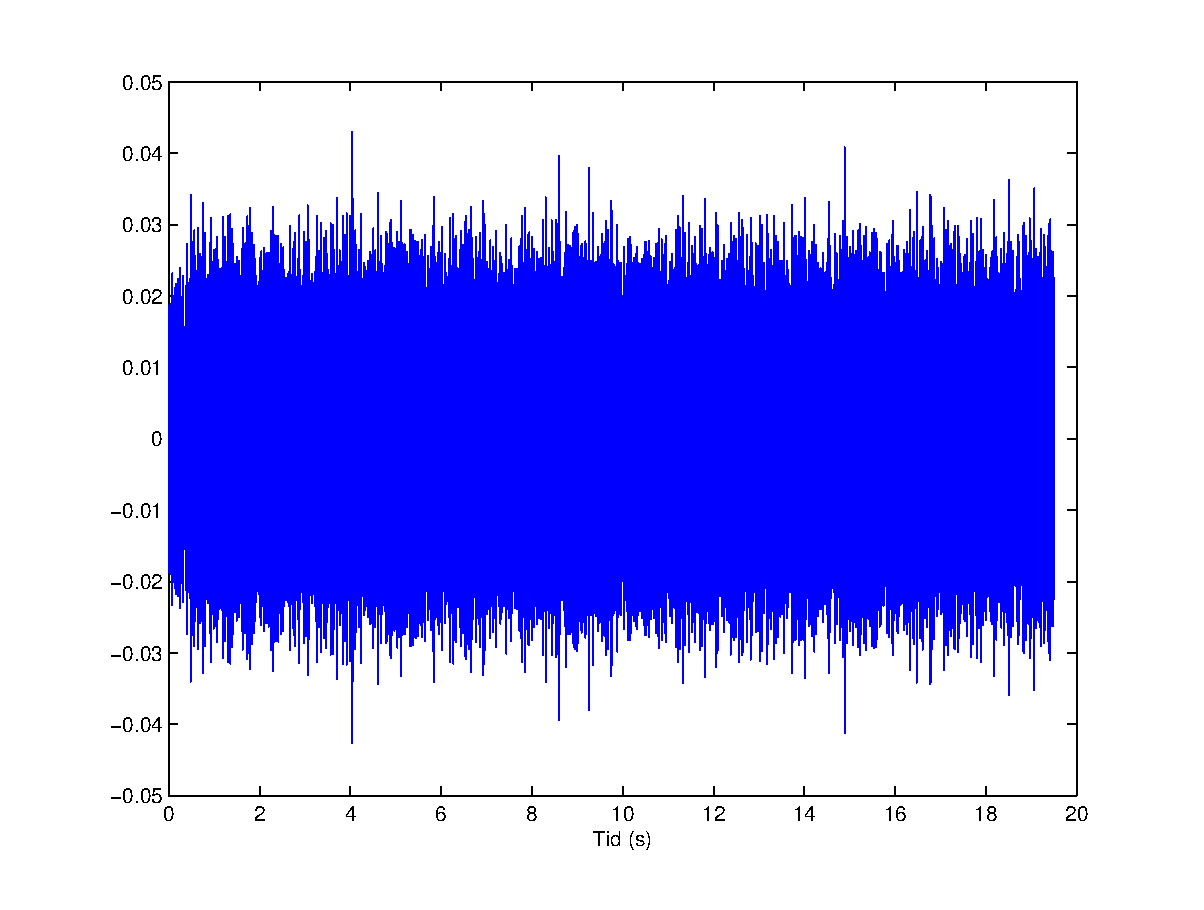
\includegraphics[keepaspectratio=true,width=\linewidth]{topp3_filter.eps}  %skala och filnamn. 
  \end{center}
  \caption{Frekvenstopp 3 filtrerad} %figurtext.
  \label{fig:topp3_filter}
\end{figure}

\newpage
\section{Kod för GNU Octave}

Fil: tsks10.m

\lstinputlisting{tsks10.m}

\newpage

Fil: playsound.m

\lstinputlisting{playsound.m}

\end{document}